\makeatletter
\def\input@path{{../styles/}{../../styles/}{../../../styles/}{../}{../../}{../../../}}
\makeatother
\documentclass{ee102_notes}
% macros.tex - Course meta information
\renewcommand{\course}{EE 102}
\renewcommand{\coursetitle}{Signal Processing and Linear Systems}
\renewcommand{\instructor}{Ayush Pandey}
\renewcommand{\semester}{Fall}
\renewcommand{\year}{2025}
\renewcommand{\shorttitle}{Week 1: Introduction to Signals}
% Use \renewcommand to avoid 'already defined' errors

% The following packages can be found on http:\\www.ctan.org
% \usepackage{graphics} % for pdf, bitmapped graphics files
%\usepackage{epsfig} % for postscript graphics files
%\usepackage{mathptmx} % assumes new font selection scheme installed
%\usepackage{times} % assumes new font selection scheme installed
\usepackage{amsmath} % assumes amsmath package installed
\usepackage{amssymb,mathtools}  % assumes amsmath package installed
\usepackage{xcolor}
\usepackage{pgfplots,subcaption}
\usepackage[hidelinks]{hyperref}
\usepackage{verbatim}
\usepackage{graphicx}
\usepackage{listings}

% -------- listings (Python) ----------
\lstdefinestyle{py}{
  language=Python,
  basicstyle=\ttfamily\small,
  keywordstyle=\color{blue!60!black}\bfseries,
  commentstyle=\color{green!40!black},
  stringstyle=\color{orange!60!black},
  showstringspaces=false,
  columns=fullflexible,
  frame=single,
  framerule=0.3pt,
  numbers=left,
  numberstyle=\tiny,
  xleftmargin=1em,
  tabsize=2,
  breaklines=true,
}
\usepackage[american]{circuitikz}
\usepackage{tikz}
\usepackage{caption}    
\usepackage{lscape}
\usepackage{soul}
\usepackage{tikz}
\usetikzlibrary{calc,angles,quotes,arrows.meta}

\usepackage{hyperref}
\hypersetup{
    colorlinks=true,
    linkcolor=blue,
    filecolor=magenta,      
    urlcolor=blue,
    pdftitle={week1_notes},
    pdfpagemode=FullScreen,
}
%\usepackage{float} 

%\usepackage[demo]{graphicx}
\pgfplotsset{compat=1.18}
% \usepgfplotslibrary{fillbetween}

\newsavebox{\measurebox}

\let\proof\relax\let\endproof\relax


\newcommand{\norm}[1]{\left\lVert#1\right\rVert}
\def\abs#1{\left\lvert#1\right\rvert}
\let\proof\relax
\let\endproof\relax
\usepackage{amsthm}
\usepackage{accents}
\usepackage{relsize}
\newcommand{\ubar}[1]{\underaccent{\bar}{#1}}
\newtheorem{theorem}{Theorem}
\newtheorem{corollary}{Corollary}[theorem]
\newtheorem{lemma}{Lemma}
\newtheorem{proposition}{Proposition}
\newtheorem{statement}{Statement}

\theoremstyle{definition}
\newtheorem{definition}{Definition}
 
\theoremstyle{remark}
\newtheorem*{remark}{Remark}
\theoremstyle{remark}
\newtheorem*{claim}{Claim}
\setlength{\parindent}{0cm}
\newenvironment{nalign}{
    \begin{equation}
    \begin{aligned}
}{
    \end{aligned}
    \end{equation}
    \ignorespacesafterend
}

\renewcommand{\releasedate}{November 17, 2025}
\newcommand{\Eblank}{\rule{3cm}{0.4pt}}
\newcommand{\Rankblank}{\rule{3cm}{0.4pt}}

\begin{document}

\begin{center}
    \textbf{EE 102: In-class activity on understanding sampling}\\[0.5em]
    \normalsize Team members: \rule{4cm}{0.15mm}\quad+\quad\rule{4cm}{0.15mm}
\end{center}

This is a two-team activity. Each team will design a sampling puzzle for the other team to solve. That is, you will provide samples of a continuous-time signal to the other team, and they will try to reconstruct the original signal from those samples. You will rate how well they did and do it again with higher number of samples. 

\noindent\textbf{Original continuous-time signal}: \(x(t) = \cos(2 \pi t) + \sin(4 \pi t)\).

\noindent\textbf{Given information}
The first component \(\cos(2 \pi t)\) has angular frequency \(\omega_1 = 2\pi\), period \(T_1 = \dfrac{2\pi}{2\pi} = 1\). Frequency in Hz is 1 Hz. The second component \(\sin(4 \pi t)\) has angular frequency \(\omega_2 = 4\pi\), period \(T_2 = \dfrac{2\pi}{4\pi} = \dfrac{1}{2}\). Frequency in Hz is 2 Hz.
So, overall signal period: \(T_0 = 1\).


\vspace{0.5em}

\noindent\textbf{Plot \(x(t)\)} Use Desmos or any other graphing tool / code to plot \(x(t)\) over the time interval \(t = 0\) to \(t = 4\). DO NOT show this plot to the other team.

\begin{center}
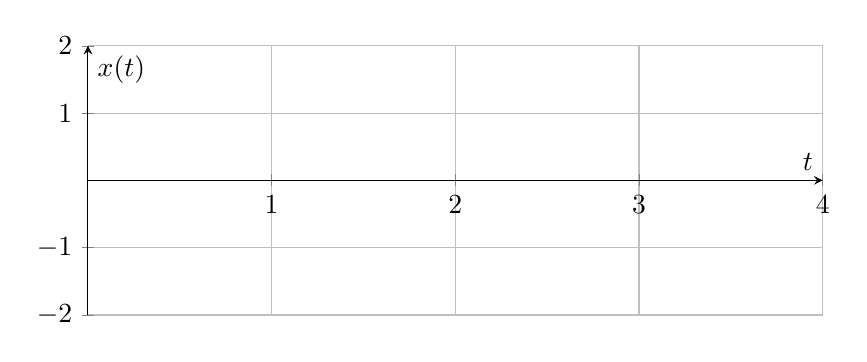
\begin{tikzpicture}
    \begin{axis}[
        width=0.9\textwidth,
        height=5cm,
        axis lines=middle,
        xlabel={$t$},
        ylabel={$x(t)$},
        xmin=0, xmax=4,
        ymin=-2, ymax=2,
        xtick={0, 1, 2, 3, 4},
        xticklabels={$0$, $1$, $2$, $3$, $4$},
        ytick={-2,-1,0,1,2},
        grid=both
    ]
    \end{axis}
\end{tikzpicture}
\end{center}

\vspace{0.5em}

\noindent\textbf{Frequency domain: }
\(
X(\omega)
= \pi\bigl[\delta(\omega-2\pi ) + \delta(\omega+2\pi )\bigr]
 - j\pi\bigl[\delta(\omega-4\pi) - \delta(\omega+4\pi)\bigr].
\)

\noindent\textbf{Sketch \(|X(\omega)|\)}: Use the axes below to sketch the locations (in \(\omega\)) of the nonzero components of \(|X(\omega)|\). You may ignore the exact complex amplitudes for now and focus on the positions at \(\omega = \pm 2\pi\) and \(\omega = \pm 4\pi\).

\begin{center}
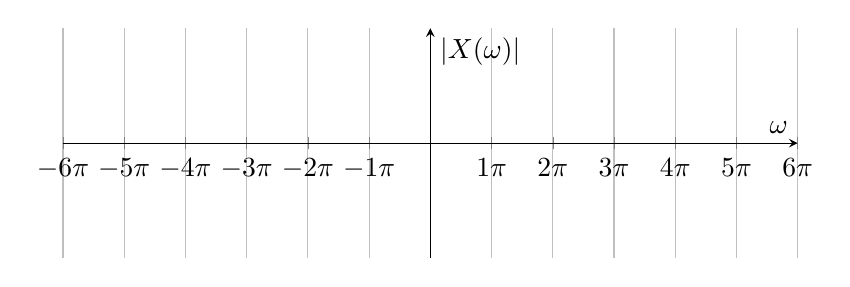
\begin{tikzpicture}
    \begin{axis}[
        width=0.9\textwidth,
        height=4.5cm,
        axis lines=middle,
        xlabel={$\omega$},
        ylabel={$|X(\omega)|$},
        xmin=-6, xmax=6,
        ymin=-1, ymax=1,
        xtick={-6,-5,-4,-3,-2,-1, 0,1, 2,3, 4,5, 6},
        xticklabels={\(-6\pi\), \(-5\pi \), \(-4\pi\), \(-3\pi\), \(-2\pi\), \(-1\pi\), \(0\), \(1\pi\), \(2\pi\), \(3\pi\), \(4\pi\), \(5\pi\), \(6\pi\)},
        ytick=\empty,
        grid=both
    ]
    % Intentionally left blank for students to draw impulses
    \end{axis}
\end{tikzpicture}
\end{center}

\newpage

\noindent\textbf{\underline{Sampling Puzzle Design \#1: Provide 8 Samples}}

You will provide 8 samples of \(x(t)\) over the \emph{fixed} time interval
\(
    t \in [0,\,4]\ \text{seconds}.
\)
Mark an ``X'' at each sample point that you provide to the other team. Place samples uniformly.

\begin{center}
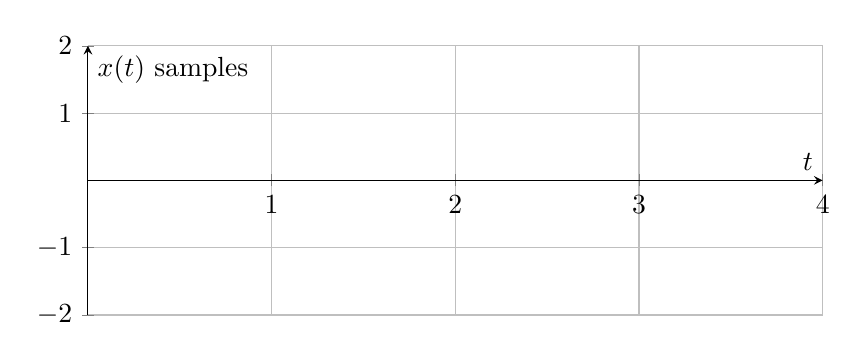
\begin{tikzpicture}
    \begin{axis}[
        width=0.9\textwidth,
        height=5cm,
        axis lines=middle,
        xlabel={$t$},
        ylabel={$x(t)$ samples},
        xmin=0, xmax=4,
        ymin=-2, ymax=2,
        xtick={0,1,2,3,4},
        xticklabels={$0$, $1$, $2$, $3$, $4$},
        ytick={-2,-1,0,1,2},
        grid=both
    ]
    % Intentionally blank: students will mark 8 samples with "X"
    \end{axis}
\end{tikzpicture}
\end{center}

Help the other team by showing them the sampling frequency computation. Since the total number of samples is \(N_1 = 8\) and the time interval is from \(t = 0\) to \(t = 4\), we have the sampling period (time between samples) (FILL IN THE BLANKS):
\[
    T_{s,1} = \frac{t_{\text{end}} - t_{\text{start}}}{N_1}
      = \rule{2cm}{0.15mm}.
\quad \text{Sampling frequency: }
    F_{s,1} = \frac{1}{T_{s,1}}
      = \rule{2cm}{0.15mm}\ \text{Hz}.
\]

Rate the reconstruction: What did you get right? \rule{2cm}{0.15mm} What did you miss? \rule{2cm}{0.15mm}

\noindent\textbf{\underline{Sampling Puzzle Design \#2: Provide 16 Samples}}

Mark an ``X'' at each sample point that you provide to the other team. Place samples uniformly. Since the total number of samples is \(N_2 = 16\) and the time interval is from \(t = 0\) to \(t = 4\), we have the sampling period (time between samples) (FILL IN THE BLANKS):
\[
    T_{s,2} = \frac{t_{\text{end}} - t_{\text{start}}}{N_2}
      = \rule{2cm}{0.15mm}.
\quad \text{Sampling frequency: }
    F_{s,2} = \frac{1}{T_{s,2}}
      = \rule{2cm}{0.15mm}\ \text{Hz}.
\]


\begin{center}
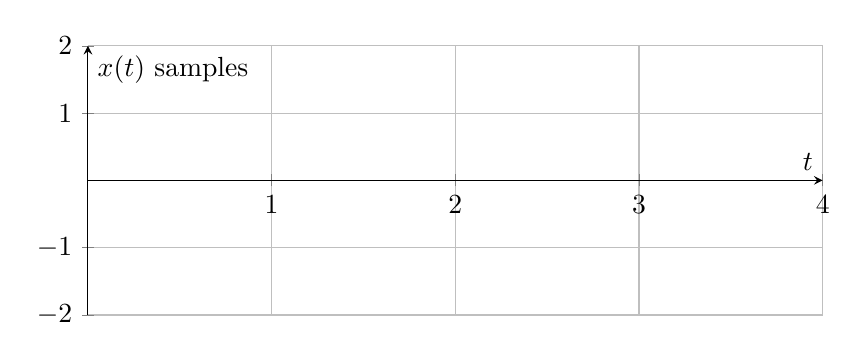
\begin{tikzpicture}
    \begin{axis}[
        width=0.9\textwidth,
        height=5cm,
        axis lines=middle,
        xlabel={$t$},
        ylabel={$x(t)$ samples},
        xmin=0, xmax=4,
        ymin=-2, ymax=2,
        xtick={0,1,2,3,4},
        xticklabels={$0$, $1$, $2$, $3$, $4$},
        ytick={-2,-1,0,1,2},
        grid=both
    ]
    % Intentionally blank: students will mark 16 samples with "X"
    \end{axis}
\end{tikzpicture}
\end{center}

Rate the reconstruction: What did you get right? \rule{2cm}{0.15mm} What did you miss? \rule{2cm}{0.15mm}
\newpage

\begin{center}
    \textbf{EE 102: In-class activity on understanding sampling}\\[0.5em]
    \normalsize Team members: \rule{4cm}{0.15mm}\quad+\quad\rule{4cm}{0.15mm}
\end{center}

This is a two-team activity. Each team will design a sampling puzzle for the other team to solve. That is, you will provide samples of a continuous-time signal to the other team, and they will try to reconstruct the original signal from those samples. You will rate how well they did and do it again with higher number of samples. 

\noindent\textbf{Original continuous-time signal}: \(x(t) = \cos(2 \pi t) + \sin(4 \pi t) + 0.8\cos(6\pi t)\).

\noindent\textbf{Given information}
The first component \(\cos(2 \pi t)\) has angular frequency \(\omega_1 = 2\pi\), period \(T_1 = \dfrac{2\pi}{2\pi} = 1\). Frequency in Hz is \(1\) Hz. The second component \(\sin(4 \pi t)\) has angular frequency \(\omega_2 = 4\pi\), period \(T_2 = \dfrac{2\pi}{4\pi} = \dfrac{1}{2}\). Frequency in Hz is \(2\) Hz. The third component \(0.8\cos(6\pi t)\) has angular frequency \(\omega_3 = 6\pi\), period \(T_3 = \dfrac{2\pi}{6\pi} = \dfrac{1}{3}\). Frequency in Hz is \(3\) Hz.

\vspace{0.5em}

\noindent\textbf{Plot \(x(t)\)} Use Desmos or any other tool to plot \(x(t)\) over \(t = 0\) to \(t = 4\). DO NOT show this plot to the other team.

\begin{center}
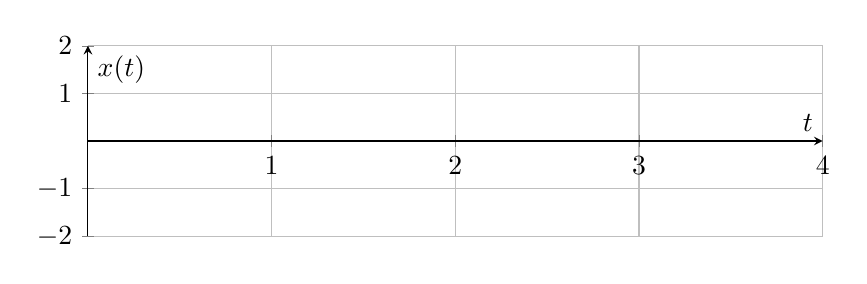
\begin{tikzpicture}
    \begin{axis}[
        width=0.9\textwidth,
        height=4cm,
        axis lines=middle,
        xlabel={$t$},
        ylabel={$x(t)$},
        xmin=0, xmax=4,
        ymin=-2, ymax=2,
        xtick={0, 1, 2, 3, 4},
        xticklabels={$0$, $1$, $2$, $3$, $4$},
        ytick={-2,-1,0,1,2},
        grid=both
    ]
    \end{axis}
\end{tikzpicture}
\end{center}

\vspace{0.5em}

\noindent\textbf{Frequency domain: }
\[
X(\omega)
= \pi\bigl[\delta(\omega-2\pi ) + \delta(\omega+2\pi )\bigr]
 - j\pi\bigl[\delta(\omega-4\pi) - \delta(\omega+4\pi)\bigr]
 + 0.8\pi\bigl[\delta(\omega-6\pi ) + \delta(\omega+6\pi )\bigr].
\]

\noindent\textbf{Sketch \(|X(\omega)|\)}: Use the axes below to sketch the locations (in \(\omega\)) of the nonzero components of \(|X(\omega)|\). Focus on the positions at \(\omega = \pm 2\pi\), \(\omega = \pm 4\pi\), and \(\omega = \pm 6\pi\).

\begin{center}
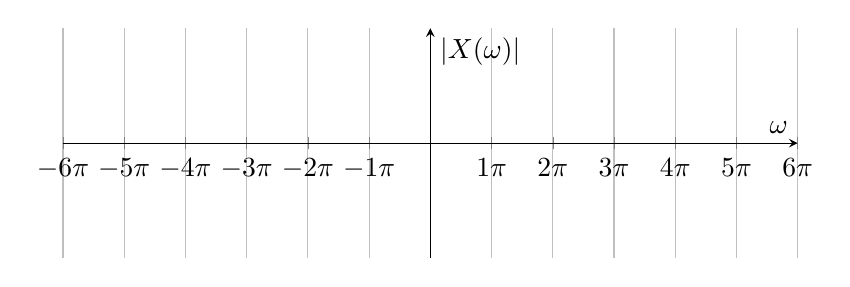
\begin{tikzpicture}
    \begin{axis}[
        width=0.9\textwidth,
        height=4.5cm,
        axis lines=middle,
        xlabel={$\omega$},
        ylabel={$|X(\omega)|$},
        xmin=-6, xmax=6,
        ymin=-1, ymax=1,
        xtick={-6,-5,-4,-3,-2,-1, 0,1, 2,3, 4,5, 6},
        xticklabels={\(-6\pi\), \(-5\pi \), \(-4\pi\), \(-3\pi\), \(-2\pi\), \(-1\pi\), \(0\), \(1\pi\), \(2\pi\), \(3\pi\), \(4\pi\), \(5\pi\), \(6\pi\)},
        ytick=\empty,
        grid=both
    ]
    % Intentionally left blank for students to draw impulses
    \end{axis}
\end{tikzpicture}
\end{center}

\newpage

\noindent\textbf{\underline{Sampling Puzzle Design \#1: Provide 8 Samples}}

You will provide 8 samples of \(x(t)\) over the \emph{fixed} time interval
\(
    t \in [0,\,4]\ \text{seconds}.
\)
Mark an ``X'' at each sample point that you provide to the other team. Place samples uniformly.

\begin{center}
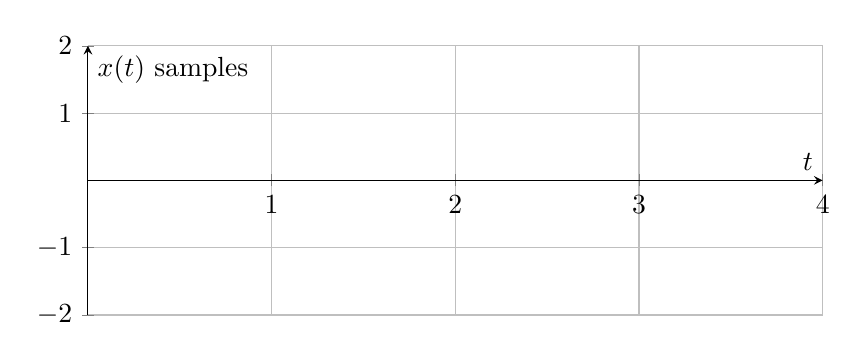
\begin{tikzpicture}
    \begin{axis}[
        width=0.9\textwidth,
        height=5cm,
        axis lines=middle,
        xlabel={$t$},
        ylabel={$x(t)$ samples},
        xmin=0, xmax=4,
        ymin=-2, ymax=2,
        xtick={0,1,2,3,4},
        xticklabels={$0$, $1$, $2$, $3$, $4$},
        ytick={-2,-1,0,1,2},
        grid=both
    ]
    % Intentionally blank: students will mark 8 samples with "X"
    \end{axis}
\end{tikzpicture}
\end{center}

Help the other team by showing them the sampling frequency computation. Since the total number of samples is \(N_1 = 8\) and the time interval is from \(t = 0\) to \(t = 4\), we have the sampling period (time between samples) (FILL IN THE BLANKS):
\[
    T_{s,1} = \frac{t_{\text{end}} - t_{\text{start}}}{N_1}
      = \rule{2cm}{0.15mm}.
\quad \text{Sampling frequency: }
    F_{s,1} = \frac{1}{T_{s,1}}
      = \rule{2cm}{0.15mm}\ \text{Hz}.
\]

Rate the reconstruction: What did you get right? \rule{2cm}{0.15mm} What did you miss? \rule{2cm}{0.15mm}

\noindent\textbf{\underline{Sampling Puzzle Design \#2: Provide 16 Samples}}

Mark an ``X'' at each sample point that you provide to the other team. Place samples uniformly. Since the total number of samples is \(N_2 = 16\) and the time interval is from \(t = 0\) to \(t = 4\), we have the sampling period (time between samples) (FILL IN THE BLANKS):
\[
    T_{s,2} = \frac{t_{\text{end}} - t_{\text{start}}}{N_2}
      = \rule{2cm}{0.15mm}.
\quad \text{Sampling frequency: }
    F_{s,2} = \frac{1}{T_{s,2}}
      = \rule{2cm}{0.15mm}\ \text{Hz}.
\]

\begin{center}
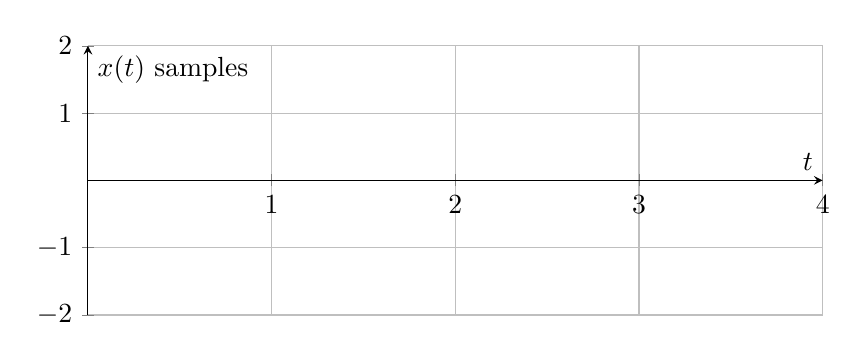
\begin{tikzpicture}
    \begin{axis}[
        width=0.9\textwidth,
        height=5cm,
        axis lines=middle,
        xlabel={$t$},
        ylabel={$x(t)$ samples},
        xmin=0, xmax=4,
        ymin=-2, ymax=2,
        xtick={0,1,2,3,4},
        xticklabels={$0$, $1$, $2$, $3$, $4$},
        ytick={-2,-1,0,1,2},
        grid=both
    ]
    % Intentionally blank: students will mark 16 samples with "X"
    \end{axis}
\end{tikzpicture}
\end{center}

Rate the reconstruction: What did you get right? \rule{2cm}{0.15mm} What did you miss? \rule{2cm}{0.15mm}

\newpage 

\begin{center}
    \textbf{EE 102: In-class activity on understanding sampling}\\[0.5em]
    \normalsize Team members: \rule{4cm}{0.15mm}\quad+\quad\rule{4cm}{0.15mm}
\end{center}

This is a two-team activity. Each team will design a sampling puzzle for the other team to solve. That is, you will provide samples of a continuous-time signal to the other team, and they will try to reconstruct the original signal from those samples. You will rate how well they did and do it again with higher number of samples. 

\noindent\textbf{Original continuous-time signal}: \(x(t) = 0.5\cos(\pi t) + \cos(2 \pi t)\).

\noindent\textbf{Given information}
The first component \(0.5\cos(\pi t)\) has angular frequency \(\omega_1 = \pi\), period \(T_1 = \dfrac{2\pi}{\pi} = 2\). Frequency in Hz is \(0.5\) Hz. The second component \(\cos(2 \pi t)\) has angular frequency \(\omega_2 = 2\pi\), period \(T_2 = \dfrac{2\pi}{2\pi} = 1\). Frequency in Hz is \(1\) Hz.
So, overall signal period: \(T_0 = 2\).

\vspace{0.5em}

\noindent\textbf{Plot \(x(t)\)} Use Desmos or any other graphing tool / code to plot \(x(t)\) over the time interval \(t = 0\) to \(t = 4\). DO NOT show this plot to the other team.

\begin{center}
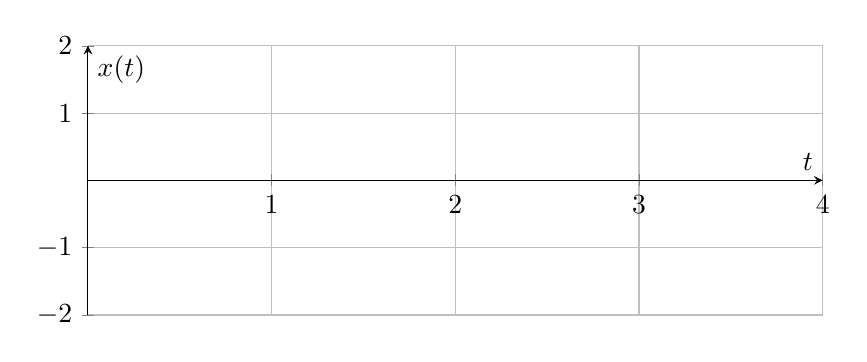
\begin{tikzpicture}
    \begin{axis}[
        width=0.9\textwidth,
        height=5cm,
        axis lines=middle,
        xlabel={$t$},
        ylabel={$x(t)$},
        xmin=0, xmax=4,
        ymin=-2, ymax=2,
        xtick={0, 1, 2, 3, 4},
        xticklabels={$0$, $1$, $2$, $3$, $4$},
        ytick={-2,-1,0,1,2},
        grid=both
    ]
    \end{axis}
\end{tikzpicture}
\end{center}

\vspace{0.5em}

\noindent\textbf{Frequency domain: }
\[
X(\omega)
= 0.5\pi\bigl[\delta(\omega-\pi ) + \delta(\omega+\pi )\bigr]
 + \pi\bigl[\delta(\omega-2\pi) + \delta(\omega+2\pi)\bigr].
\]

\noindent\textbf{Sketch \(|X(\omega)|\)}: Use the axes below to sketch the locations (in \(\omega\)) of the nonzero components of \(|X(\omega)|\). Focus on the positions at \(\omega = \pm \pi\) and \(\omega = \pm 2\pi\).

\begin{center}
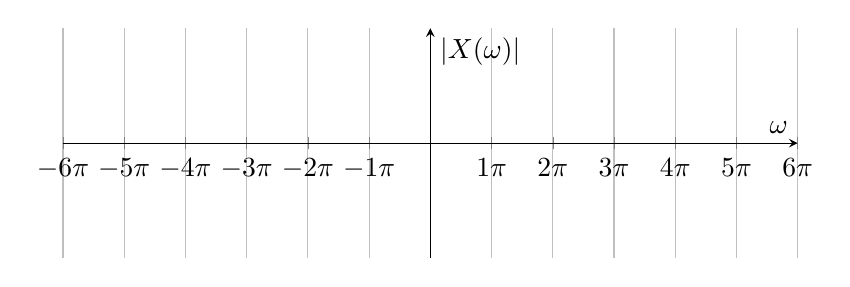
\begin{tikzpicture}
    \begin{axis}[
        width=0.9\textwidth,
        height=4.5cm,
        axis lines=middle,
        xlabel={$\omega$},
        ylabel={$|X(\omega)|$},
        xmin=-6, xmax=6,
        ymin=-1, ymax=1,
        xtick={-6,-5,-4,-3,-2,-1, 0,1, 2,3, 4,5, 6},
        xticklabels={\(-6\pi\), \(-5\pi \), \(-4\pi\), \(-3\pi\), \(-2\pi\), \(-1\pi\), \(0\), \(1\pi\), \(2\pi\), \(3\pi\), \(4\pi\), \(5\pi\), \(6\pi\)},
        ytick=\empty,
        grid=both
    ]
    % Intentionally left blank for students to draw impulses
    \end{axis}
\end{tikzpicture}
\end{center}

\newpage

\noindent\textbf{\underline{Sampling Puzzle Design \#1: Provide 8 Samples}}

You will provide 8 samples of \(x(t)\) over the \emph{fixed} time interval
\(
    t \in [0,\,4]\ \text{seconds}.
\)
Mark an ``X'' at each sample point that you provide to the other team. Place samples uniformly.

\begin{center}
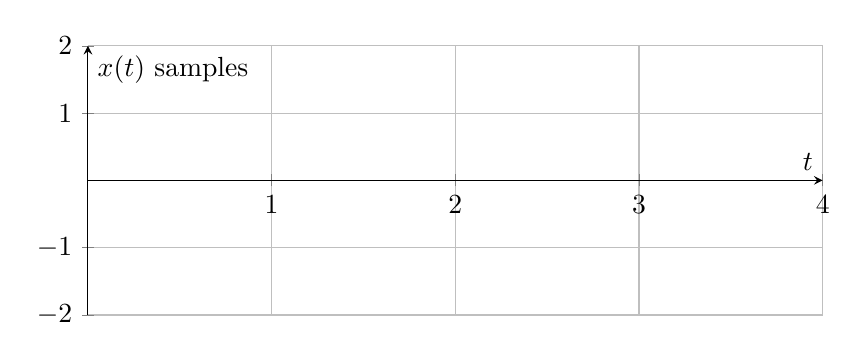
\begin{tikzpicture}
    \begin{axis}[
        width=0.9\textwidth,
        height=5cm,
        axis lines=middle,
        xlabel={$t$},
        ylabel={$x(t)$ samples},
        xmin=0, xmax=4,
        ymin=-2, ymax=2,
        xtick={0,1,2,3,4},
        xticklabels={$0$, $1$, $2$, $3$, $4$},
        ytick={-2,-1,0,1,2},
        grid=both
    ]
    % Intentionally blank: students will mark 8 samples with "X"
    \end{axis}
\end{tikzpicture}
\end{center}

Help the other team by showing them the sampling frequency computation. Since the total number of samples is \(N_1 = 8\) and the time interval is from \(t = 0\) to \(t = 4\), we have the sampling period (time between samples) (FILL IN THE BLANKS):
\[
    T_{s,1} = \frac{t_{\text{end}} - t_{\text{start}}}{N_1}
      = \rule{2cm}{0.15mm}.
\quad \text{Sampling frequency: }
    F_{s,1} = \frac{1}{T_{s,1}}
      = \rule{2cm}{0.15mm}\ \text{Hz}.
\]

Rate the reconstruction: What did you get right? \rule{2cm}{0.15mm} What did you miss? \rule{2cm}{0.15mm}

\noindent\textbf{\underline{Sampling Puzzle Design \#2: Provide 16 Samples}}

Mark an ``X'' at each sample point that you provide to the other team. Place samples uniformly. Since the total number of samples is \(N_2 = 16\) and the time interval is from \(t = 0\) to \(t = 4\), we have the sampling period (time between samples) (FILL IN THE BLANKS):
\[
    T_{s,2} = \frac{t_{\text{end}} - t_{\text{start}}}{N_2}
      = \rule{2cm}{0.15mm}.
\quad \text{Sampling frequency: }
    F_{s,2} = \frac{1}{T_{s,2}}
      = \rule{2cm}{0.15mm}\ \text{Hz}.
\]

\begin{center}
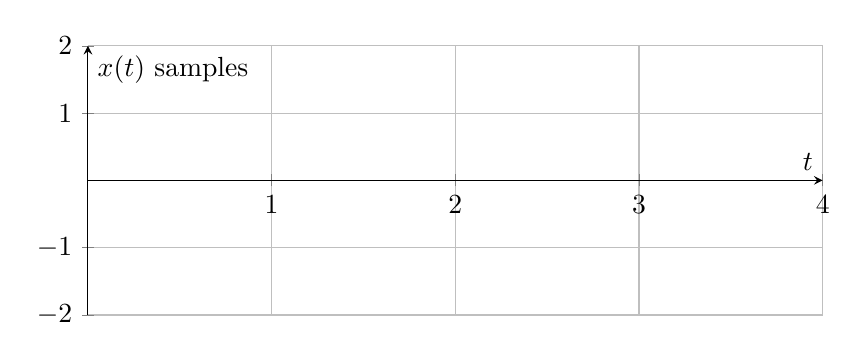
\begin{tikzpicture}
    \begin{axis}[
        width=0.9\textwidth,
        height=5cm,
        axis lines=middle,
        xlabel={$t$},
        ylabel={$x(t)$ samples},
        xmin=0, xmax=4,
        ymin=-2, ymax=2,
        xtick={0,1,2,3,4},
        xticklabels={$0$, $1$, $2$, $3$, $4$},
        ytick={-2,-1,0,1,2},
        grid=both
    ]
    % Intentionally blank: students will mark 16 samples with "X"
    \end{axis}
\end{tikzpicture}
\end{center}

Rate the reconstruction: What did you get right? \rule{2cm}{0.15mm} What did you miss? \rule{2cm}{0.15mm}

\newpage

\begin{center}
    \textbf{EE 102: In-class activity on understanding sampling}\\[0.5em]
    \normalsize Team members: \rule{4cm}{0.15mm}\quad+\quad\rule{4cm}{0.15mm}
\end{center}

This is a two-team activity. Each team will design a sampling puzzle for the other team to solve. That is, you will provide samples of a continuous-time signal to the other team, and they will try to reconstruct the original signal from those samples. You will rate how well they did and do it again with higher number of samples. 

\noindent\textbf{Original continuous-time signal}: \(x(t) = \cos(2 \pi t) + \sin(3 \pi t)\).

\noindent\textbf{Given information}
The first component \(\cos(2 \pi t)\) has angular frequency \(\omega_1 = 2\pi\), period \(T_1 = \dfrac{2\pi}{2\pi} = 1\). Frequency in Hz is \(1\) Hz. The second component \(\sin(3 \pi t)\) has angular frequency \(\omega_2 = 3\pi\), period \(T_2 = \dfrac{2\pi}{3\pi} = \dfrac{2}{3}\). Frequency in Hz is \(1.5\) Hz.
So, overall signal period: \(T_0 = 2\).

\vspace{0.5em}

\noindent\textbf{Plot \(x(t)\)} Use Desmos or any other graphing tool / code to plot \(x(t)\) over the time interval \(t = 0\) to \(t = 4\). DO NOT show this plot to the other team.

\begin{center}
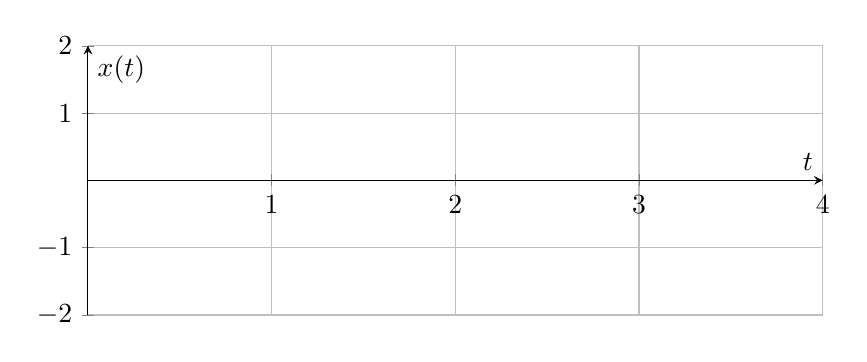
\begin{tikzpicture}
    \begin{axis}[
        width=0.9\textwidth,
        height=5cm,
        axis lines=middle,
        xlabel={$t$},
        ylabel={$x(t)$},
        xmin=0, xmax=4,
        ymin=-2, ymax=2,
        xtick={0, 1, 2, 3, 4},
        xticklabels={$0$, $1$, $2$, $3$, $4$},
        ytick={-2,-1,0,1,2},
        grid=both
    ]
    \end{axis}
\end{tikzpicture}
\end{center}

\vspace{0.5em}

\noindent\textbf{Frequency domain: }
\[
X(\omega)
= \pi\bigl[\delta(\omega-2\pi ) + \delta(\omega+2\pi )\bigr]
 - j\pi\bigl[\delta(\omega-3\pi) - \delta(\omega+3\pi)\bigr].
\]

\noindent\textbf{Sketch \(|X(\omega)|\)}: Use the axes below to sketch the locations (in \(\omega\)) of the nonzero components of \(|X(\omega)|\). Focus on the positions at \(\omega = \pm 2\pi\) and \(\omega = \pm 3\pi\).

\begin{center}
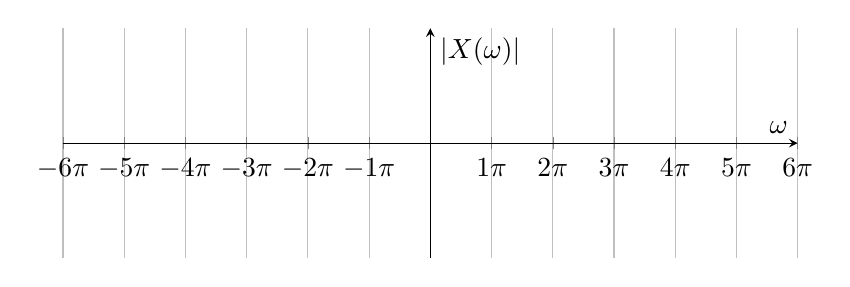
\begin{tikzpicture}
    \begin{axis}[
        width=0.9\textwidth,
        height=4.5cm,
        axis lines=middle,
        xlabel={$\omega$},
        ylabel={$|X(\omega)|$},
        xmin=-6, xmax=6,
        ymin=-1, ymax=1,
        xtick={-6,-5,-4,-3,-2,-1, 0,1, 2,3, 4,5, 6},
        xticklabels={\(-6\pi\), \(-5\pi \), \(-4\pi\), \(-3\pi\), \(-2\pi\), \(-1\pi\), \(0\), \(1\pi\), \(2\pi\), \(3\pi\), \(4\pi\), \(5\pi\), \(6\pi\)},
        ytick=\empty,
        grid=both
    ]
    % Intentionally left blank for students to draw impulses
    \end{axis}
\end{tikzpicture}
\end{center}

\newpage

\noindent\textbf{\underline{Sampling Puzzle Design \#1: Provide 8 Samples}}

You will provide 8 samples of \(x(t)\) over the \emph{fixed} time interval
\(
    t \in [0,\,4]\ \text{seconds}.
\)
Mark an ``X'' at each sample point that you provide to the other team. Place samples uniformly.

\begin{center}
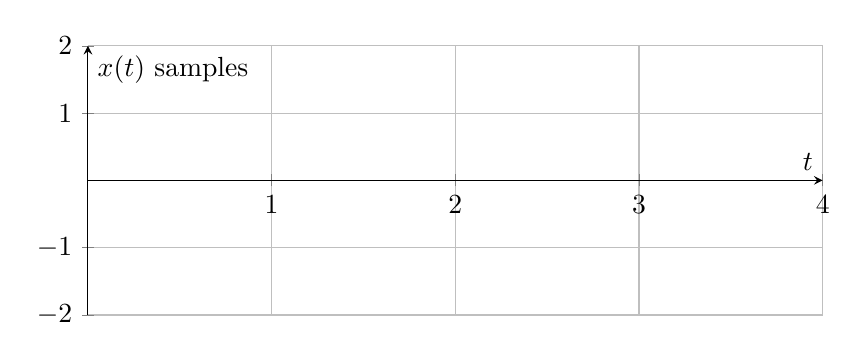
\begin{tikzpicture}
    \begin{axis}[
        width=0.9\textwidth,
        height=5cm,
        axis lines=middle,
        xlabel={$t$},
        ylabel={$x(t)$ samples},
        xmin=0, xmax=4,
        ymin=-2, ymax=2,
        xtick={0,1,2,3,4},
        xticklabels={$0$, $1$, $2$, $3$, $4$},
        ytick={-2,-1,0,1,2},
        grid=both
    ]
    % Intentionally blank: students will mark 8 samples with "X"
    \end{axis}
\end{tikzpicture}
\end{center}

Help the other team by showing them the sampling frequency computation. Since the total number of samples is \(N_1 = 8\) and the time interval is from \(t = 0\) to \(t = 4\), we have the sampling period (time between samples) (FILL IN THE BLANKS):
\[
    T_{s,1} = \frac{t_{\text{end}} - t_{\text{start}}}{N_1}
      = \rule{2cm}{0.15mm}.
\quad \text{Sampling frequency: }
    F_{s,1} = \frac{1}{T_{s,1}}
      = \rule{2cm}{0.15mm}\ \text{Hz}.
\]

Rate the reconstruction: What did you get right? \rule{2cm}{0.15mm} What did you miss? \rule{2cm}{0.15mm}

\noindent\textbf{\underline{Sampling Puzzle Design \#2: Provide 16 Samples}}

Mark an ``X'' at each sample point that you provide to the other team. Place samples uniformly. Since the total number of samples is \(N_2 = 16\) and the time interval is from \(t = 0\) to \(t = 4\), we have the sampling period (time between samples) (FILL IN THE BLANKS):
\[
    T_{s,2} = \frac{t_{\text{end}} - t_{\text{start}}}{N_2}
      = \rule{2cm}{0.15mm}.
\quad \text{Sampling frequency: }
    F_{s,2} = \frac{1}{T_{s,2}}
      = \rule{2cm}{0.15mm}\ \text{Hz}.
\]

\begin{center}
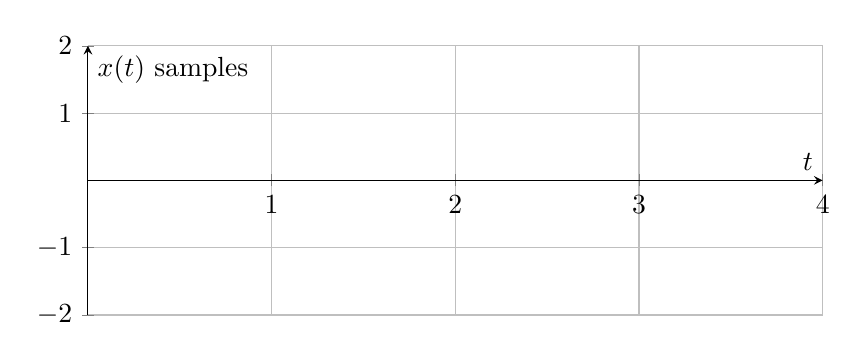
\begin{tikzpicture}
    \begin{axis}[
        width=0.9\textwidth,
        height=5cm,
        axis lines=middle,
        xlabel={$t$},
        ylabel={$x(t)$ samples},
        xmin=0, xmax=4,
        ymin=-2, ymax=2,
        xtick={0,1,2,3,4},
        xticklabels={$0$, $1$, $2$, $3$, $4$},
        ytick={-2,-1,0,1,2},
        grid=both
    ]
    % Intentionally blank: students will mark 16 samples with "X"
    \end{axis}
\end{tikzpicture}
\end{center}

Rate the reconstruction: What did you get right? \rule{2cm}{0.15mm} What did you miss? \rule{2cm}{0.15mm}


\end{document}